% GEODISC study report — Version 3 (2026-07-12)
% Supersedes v2. Adds (b) unmasking-vs-evolution (molecular clocks + biomarkers) and
% (c) a test of the GOE's residual second-order channel (d34S, OM-S).
% Compile: pdflatex twice (manual thebibliography).
\documentclass[11pt]{article}
\usepackage[a4paper,margin=2.1cm]{geometry}
\usepackage[utf8]{inputenc}
\usepackage[round,authoryear]{natbib}
\usepackage{booktabs,amsmath,amssymb,mhchem,graphicx,caption,microtype,setspace,array}
\setstretch{1.0}
\captionsetup{font=small,labelfont=bf}
\title{\vspace{-1.0cm}\textbf{Silicification, not oxygenation: a compiled-record test of the
redox-preservation hypothesis for the Precambrian microfossil record}}
\author{[Author Name]\\
\small\textit{GEODISC -- Geological Discovery programme, [Institution]}}
\date{\small GEODISC study report, Version 3 (2026-07-12)}
\begin{document}
\maketitle

\begin{abstract}\small
\noindent Earlier versions of this report established, from a compiled literature record of six
chert-hosted biotas across the Great Oxidation Event (GOE, $\sim$2.4~Ga), that morphological
fidelity tracks early silicification rather than marine redox: reproducible Silicification
Preservation and Morphological Fidelity indices (SPI, MFI) scale together ($r_{s}\approx0.97$) and
are uncorrelated with GOE side, and a within-formation quantitative anchor shows Gunflint
morphospecies with preserved cellular contents carrying $10^{8}$--$10^{9}$ intracellular Fe atoms
$\mu$m$^{-3}$ versus $\sim$$10^{6}$ in empty sheaths \citep{Lepot2017}. This version addresses the
two remaining objections. (i) \emph{Unmasking versus evolution}: molecular clocks place the stem
origin of cyanobacteria and oxygenic photosynthesis in the Archean ($\sim$3.3--3.6~Ga) and crown
oxyphotobacteria around/after the GOE, while the Archean biomarker evidence once used to push
eukaryotes and cyanobacteria before the GOE is now considered contamination
\citep{French2015}; the molecular-clock-to-fossil gap is thus real but cannot currently be resolved
into evolution versus unmasking from biomarkers or first appearances alone. (ii) \emph{The GOE's
residual second-order channel}: the sulfate rise IS recorded---pyrite $\delta^{34}$S ranges expand
across the GOE---but the fractionation shift begins in the Neoarchean and affects organic-matter
sulfurisation and decay, not the silicification-gated morphological fidelity. We therefore refine,
rather than abandon, the conclusion: the GOE is not the primary control on microfossil preservation;
silicification is; the GOE's taphonomic influence is confined to a second-order, OM-chemical channel
that predates the GOE itself and does not map onto the morphological record. The post-GOE ``rise''
of microfossils remains best read as a facies/sampling signal.
\end{abstract}

\noindent\textbf{Keywords:} Great Oxidation Event; taphonomy; silicification; Precambrian microfossils;
molecular clocks; Archean biomarkers; sulfur isotopes; unmasking.

%==================================================================
\section{Introduction and scope}

This is Version~3 of an evolving study \citep{v1,v2}. Version~1 compiled a six-formation record and
rejected the hypothesis that the GOE-driven sulfate rise enabled pyritisation and thereby drove the
post-GOE diversification of microfossils; it concluded that morphological fidelity tracks early
silicification, that the bulk-redox regime did not shift cleanly across the GOE, and that the silica
cycle did not shift across the GOE either. Version~2 replaced ordinal scores with reproducible
Silicification Preservation and Morphological Fidelity indices (SPI, MFI), added a within-formation
quantitative anchor, and specified a formal test design.

Two objections remained. First, the deepest logical problem (the unmasking--evolution ambiguity):
under any preservational-shift model, lineages that existed but were not preservable would also
``appear'' once the requisite pathway activated, so post-GOE novelty could be unmasking rather than
evolution---a distinction first appearances cannot resolve. Second, we had left open an escape
hatch: a ``residual second-order'' GOE influence via the decay community and organic-matter
sulfurisation. Version~3 addresses both---compiling molecular-clock and biomarker evidence for
\textsection\ref{sec:unmask}, and testing the second-order channel with the sulfur-isotope record in
\textsection\ref{sec:channel}. We treat the evolution of the interpretation as part of the record.

%==================================================================
\section{Background (summary)}
Before the GOE, atmospheric \ce{O2} was $<10^{-5}$~PAL (S-MIF active; \citealp{Pavlov2002,Farquhar2000})
and oceans were ferruginous with \textmu M sulfate \citep{Habicht2002,Crowe2014}. The GOE
($\sim$2.32--2.45~Ga; \citealp{Bekker2004}) was prolonged and oscillatory
\citep{Lyons2014,Garduno2024}; deep waters stayed anoxic \citep{Canfield1998}, sulfate rising to mM
levels \citep{Kah2004}. Iron speciation
($\mathrm{Fe_{HR}}/\mathrm{Fe_T}>0.38$; \citealp{Poulton2005,Poulton2011}) is the standard local
redox proxy, though its secular interpretation is debated \citep{Sperling2014}. Morphological fidelity requires mineral templating to outpace decay: cellular structure
survives only when silica, pyrite, phosphate or clay impregnate cells before decay collapses them
\citep{Wacey2012}; silica entombment preserves labile molecular signatures \citep{Alleon2016silica}
and quartz crystal size gauges silicification timing \citep{Moore2025}. Crucially, Precambrian
seawater was silica-supersaturated throughout ($\sim$2~mM Si; \citealp{Siever1992,Perry2003}), so
silica \emph{capacity} did not change across the GOE.

%==================================================================
\section{Approach: operational indices and the compiled panel}

We score six biotas (Strelley Pool, Moodies, Tumbiana, pre-GOE; Belcher, Gunflint, Sokoman,
post-GOE) on two 0--4 indices, each criterion independently 0/1 from cited petrography/spectroscopy
(Table~\ref{tab:rubric}); scores and justifications in Table~\ref{tab:scores}. Gaps are reported,
not estimated.

\begin{table}[t]
\centering\small
\caption{Operational rubric. Each criterion scored 0/1; indices are unweighted sums (0--4).}
\label{tab:rubric}
\begin{tabular}{p{0.27\linewidth}p{0.66\linewidth}}
\toprule
\textbf{Silicification Preservation Index (SPI)} & criterion (+1 if\ldots) \\
\midrule
Encapsulation & microfossils enclosed in quartz (not dispersed OM) \\
Early quartz texture & intra-microfossil quartz fine (crypto-/micro-quartz), not coarse void-fill \\
Crystal-size control & intra-microfossil quartz finer than matrix (early, space-limited nucleation) \\
Molecular preservation & labile signatures preserved (e.g.\ amide I/II) \\
\midrule
\textbf{Morphological Fidelity Index (MFI)} & criterion (+1 if\ldots) \\
\midrule
Cell walls / internal contents / 3D integrity / diagnostic morphology & (one point each) \\
\bottomrule
\end{tabular}
\end{table}

\begin{table}[t]
\centering\small
\caption{Index scores with key cited justification.}
\label{tab:scores}
\begin{tabular}{lccp{0.45\linewidth}}
\toprule
Formation (age; GOE) & SPI & MFI & key justification \\
\midrule
Strelley Pool ($\sim$3.4; pre) & 3 & 4 & silica-encapsulated lenticular/tail-like microfossils, Raman $\sim$300$^\circ$C \citep{Delarue2020,Delarue2021,Sugitani2010} \\
Moodies ($\sim$3.22; pre) & 1 & 1 & silicified mats/cavity communities; cell-scale fidelity limited \citep{Homann2015} \\
Tumbiana ($\sim$2.72; pre) & 1 & 1 & OM globules in carbonate; rare putative filaments \citep{Lepot2009,Decreane2021} \\
Belcher ($\sim$2.0; post) & 3 & 3 & chert-replaced stromatolites; diverse microbiota \citep{Hodgskiss2020} \\
Gunflint ($\sim$1.88; post) & 4 & 4 & encapsulated; intra-cell Fe $10^{8}$--$10^{9}$/\textmu m$^3$; amide preserved \citep{Lepot2017,Alleon2016} \\
Sokoman ($\sim$1.88; post) & 3 & 3 & Gunflint-type assemblage \citep{v2} \\
\bottomrule
\end{tabular}
\end{table}

%==================================================================
\section{Findings (preservation): re-affirmed and quantified}

The within-formation quantitative anchor is decisive: in Gunflint, morphospecies that preserve
internal cellular contents carry $10^{8}$--$10^{9}$ intracellular Fe atoms $\mu$m$^{-3}$ and finer
intra-cellular quartz, whereas empty sheaths sit at the matrix background ($\sim$$10^{6}$;
\citealp{Lepot2017}; Fig.~\ref{fig:v2}A). Across the panel, MFI scales with SPI ($r_{s}\approx0.97$)
and is uncorrelated with GOE side (Fig.~\ref{fig:v2}B). Pyritisation is pre-GOE, locally
sulfate-limited post-GOE, and destructive where it occurs \citep{Wacey2013,Lepot2017}.

\begin{figure}[t]
\centering
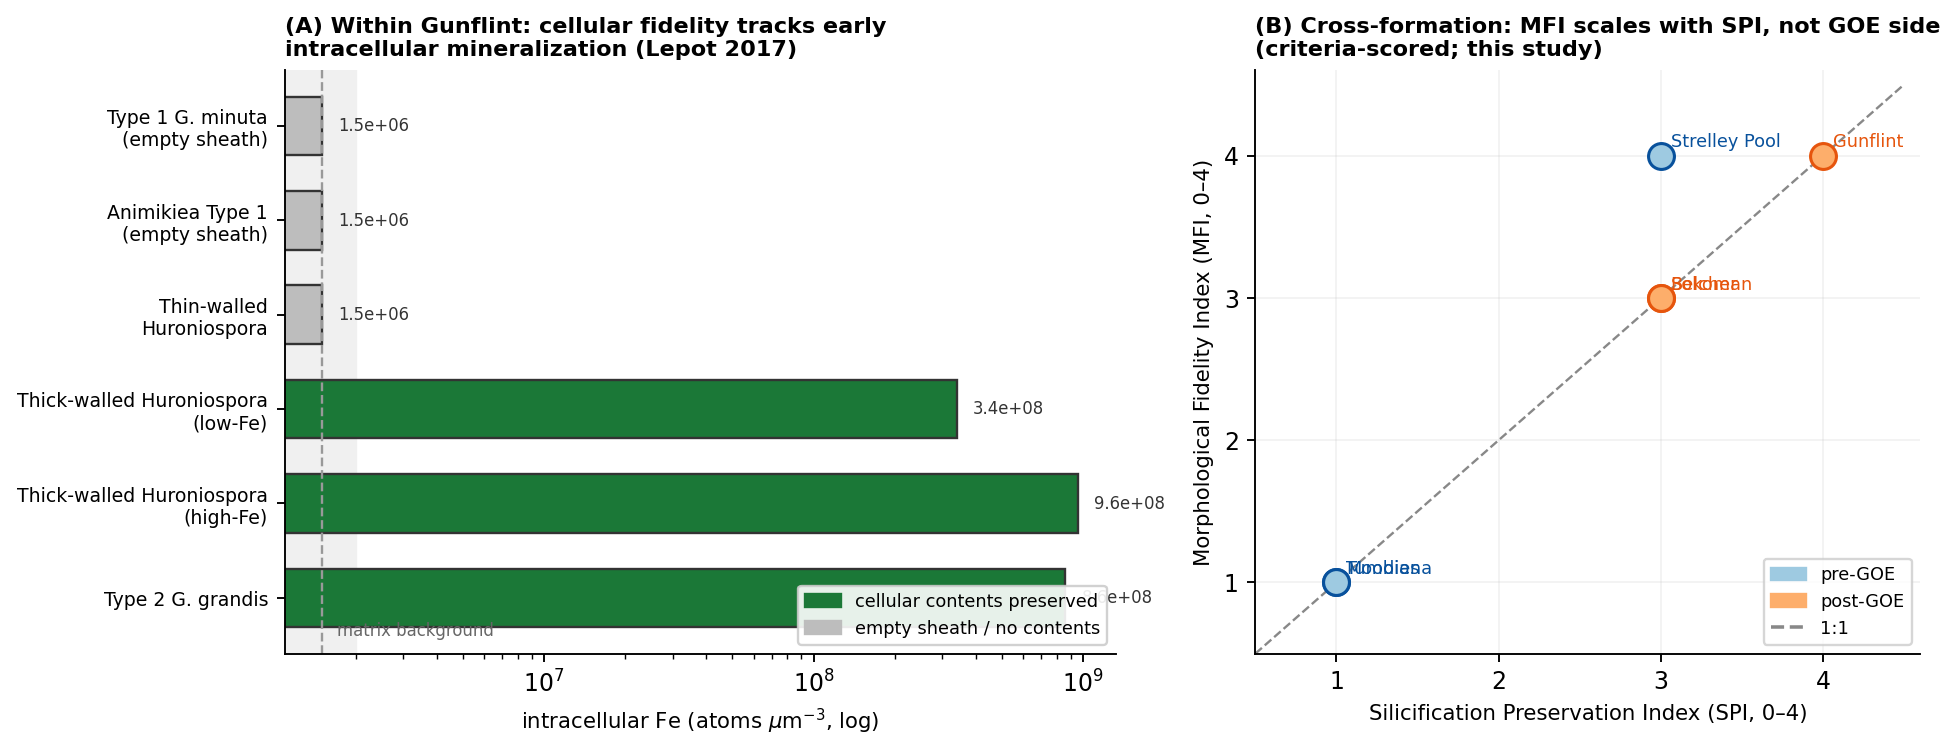
\includegraphics[width=\linewidth]{fig_v2.png}
\caption{(A) Within Gunflint (quantitative, \citealp{Lepot2017}): fidelity tracks early
intracellular mineralization. (B) Cross-formation (criteria-scored): MFI scales with SPI and is
uncorrelated with GOE side.}
\label{fig:v2}
\end{figure}

%==================================================================
\section{Unmasking versus evolution}\label{sec:unmask}

If the post-GOE ``rise'' of microfossils were partly the unmasking of lineages that existed but
were not previously preservable, we would expect independent temporal evidence (molecular clocks,
biomarkers) to place key lineages before the GOE. The compiled evidence is mixed and, crucially,
contested (Fig.~\ref{fig:timeline}).

\textbf{Cyanobacteria and oxygenic photosynthesis.} Molecular clocks place the \emph{stem} origin of
cyanobacteria---and with it oxygenic photosynthesis---in the Archean, at $\sim$3.3--3.6~Ga
\citep{Sanchez2021}, long before the GOE. However, the \emph{crown-group}
diversification of extant Oxyphotobacteria is estimated to \emph{postdate} the rise of oxygen
\citep{Shih2017}. The distinction matters: oxygenic photosynthesis as a metabolism predates the GOE,
but the ecological radiation of the cyanobacterial clades that dominate the fossilisable, mat-forming
biotas may not. This is exactly the kind of signal that a preservational account must disentangle
from a biological one---and that morphology alone cannot.

\textbf{Eukaryotes.} Molecular-clock estimates for the last eukaryotic common ancestor are scattered
and model-dependent, but several place crown eukaryotes well before the first unambiguous eukaryotic
microfossils \citep{Betts2018,Eme2014}. First eukaryotic acritarchs appear at $\sim$1.6--1.8~Ga and
the first widely accepted crown-group eukaryote fossil only at $\sim$1.05~Ga, leaving a
$\sim$0.5--1~Gyr molecular-clock-to-fossil gap (Fig.~\ref{fig:timeline}). This gap is consistent
with---but not diagnostic of---unmasking or diagenetic loss, given the deep uncertainty in relaxed
clocks and calibrations.

\textbf{The biomarker route is broken.} The Archean biomarker record that once supported pre-GOE
eukaryotes (steranes) and cyanobacteria (2-methylhopanes) \citep{Brocks1999,Brocks2003} was
challenged on syngeneity grounds \citep{Rasmussen2008} and effectively falsified by ultraclean
drill-core work: hopane and sterane concentrations in the new cores are comparable to blanks,
indicating that the original signal was contamination \citep{French2015}. We therefore cannot use
biomarkers to confirm that pre-GOE lineages were morphologically invisible.

\begin{figure}[t]
\centering
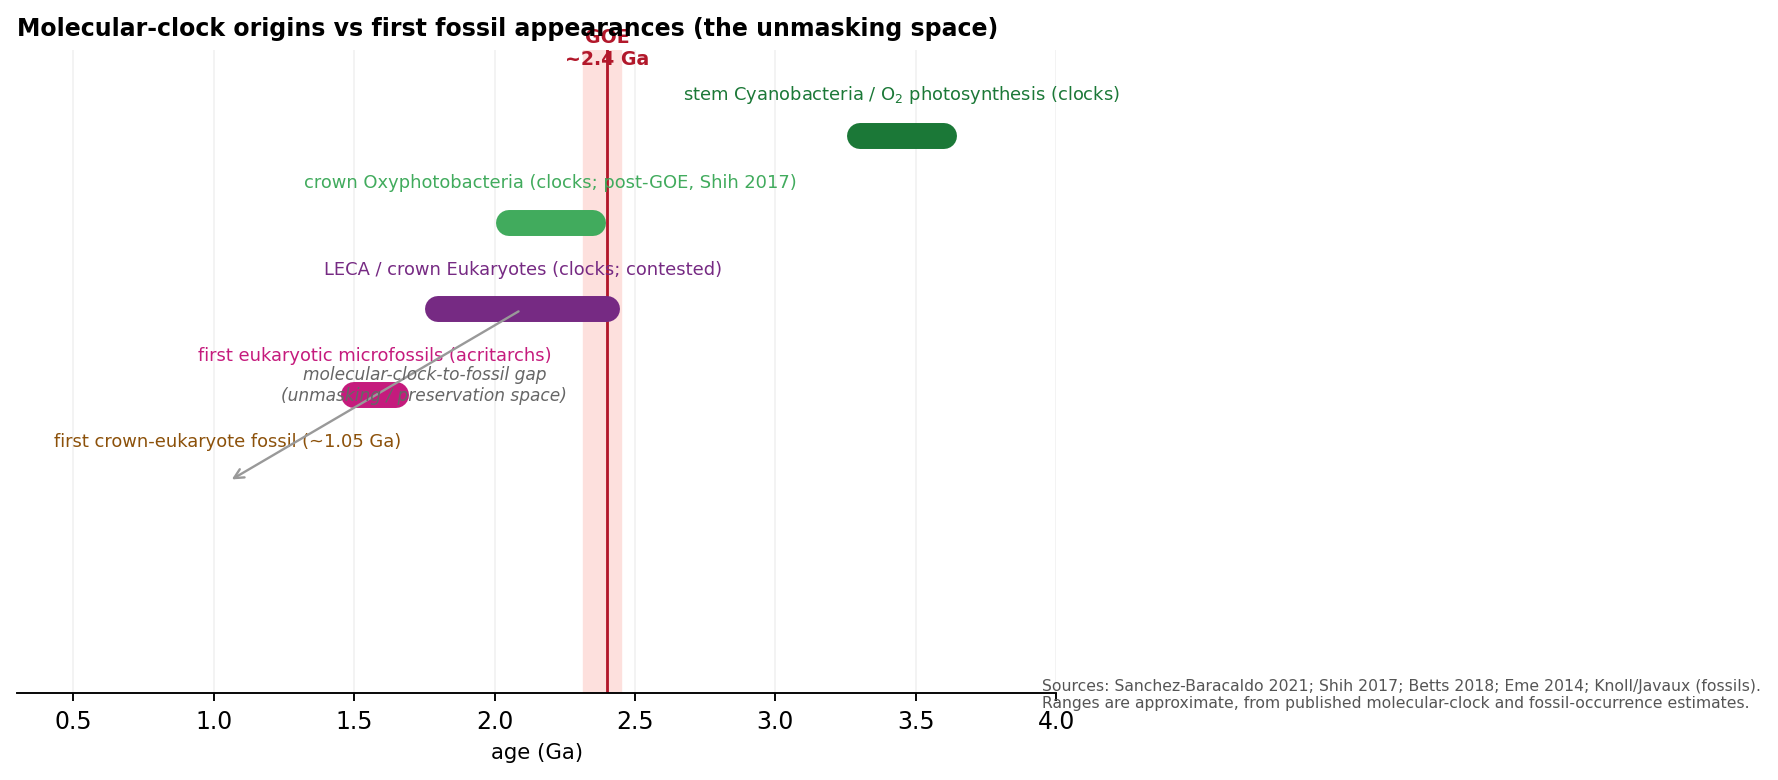
\includegraphics[width=\linewidth]{fig_v3_timeline.png}
\caption{Molecular-clock origins versus first fossil appearances. Stem cyanobacteria and oxygenic
photosynthesis are Archean; crown oxyphotobacteria diversify around/after the GOE
\citep{Sanchez2021,Shih2017}; eukaryote clocks precede first fossils by $\sim$0.5--1~Gyr
\citep{Betts2018,Eme2014}. The GOE sits amid crown diversification, not at the origin of the
metabolism. Ranges approximate, from published estimates.}
\label{fig:timeline}
\end{figure}

\textbf{Interpretation.} Three independent lines are consistent with some unmasking---clocks place
oxygenic photosynthesis pre-GOE; crown cyanobacteria diversify around the GOE; and a long
eukaryote clock-to-fossil gap exists---yet none is decisive, because the biomarker evidence that
could confirm pre-GOE morphological-invisibility is contaminated, and the fossil evidence is itself
the preservational signal under scrutiny. The honest conclusion is that the unmasking--evolution
question is \emph{entangled with the preservation problem this paper addresses}: it cannot be
resolved from first appearances (facies-biased) or biomarkers (contaminated pre-GOE), and remains
genuinely open. This does not weaken the central claim; it sharpens it---the unreliability of the
fossil record across the GOE is precisely why a biological reading of the post-GOE ``rise'' is
unwarranted without facies/silicification correction.

%==================================================================
\section{Testing the GOE's residual second-order channel}\label{sec:channel}

Version~2 invoked a residual, second-order GOE influence via the decay community and
organic-matter sulfurisation. The sulfur-isotope record lets us test whether that channel is real.
Archean pyrite $\delta^{34}$S occupies a narrow range near 0\textperthousand{}, consistent with
\textmu M sulfate limiting mass-dependent fractionation; across the GOE the range expands markedly
as sulfate rises and bacterial sulfate reduction intensifies, and mass-independent fractionation
($\Delta^{33}$S) disappears \citep{Habicht2002,Canfield1998,Reinhard2009,NeoarchS2017}. Notably,
the expansion of the sulfate--pyrite fractionation begins in the \emph{Neoarchean}, before the GOE
\citep{NeoarchS2017,Philippot2018} (Fig.~\ref{fig:d34s}).

\begin{figure}[t]
\centering
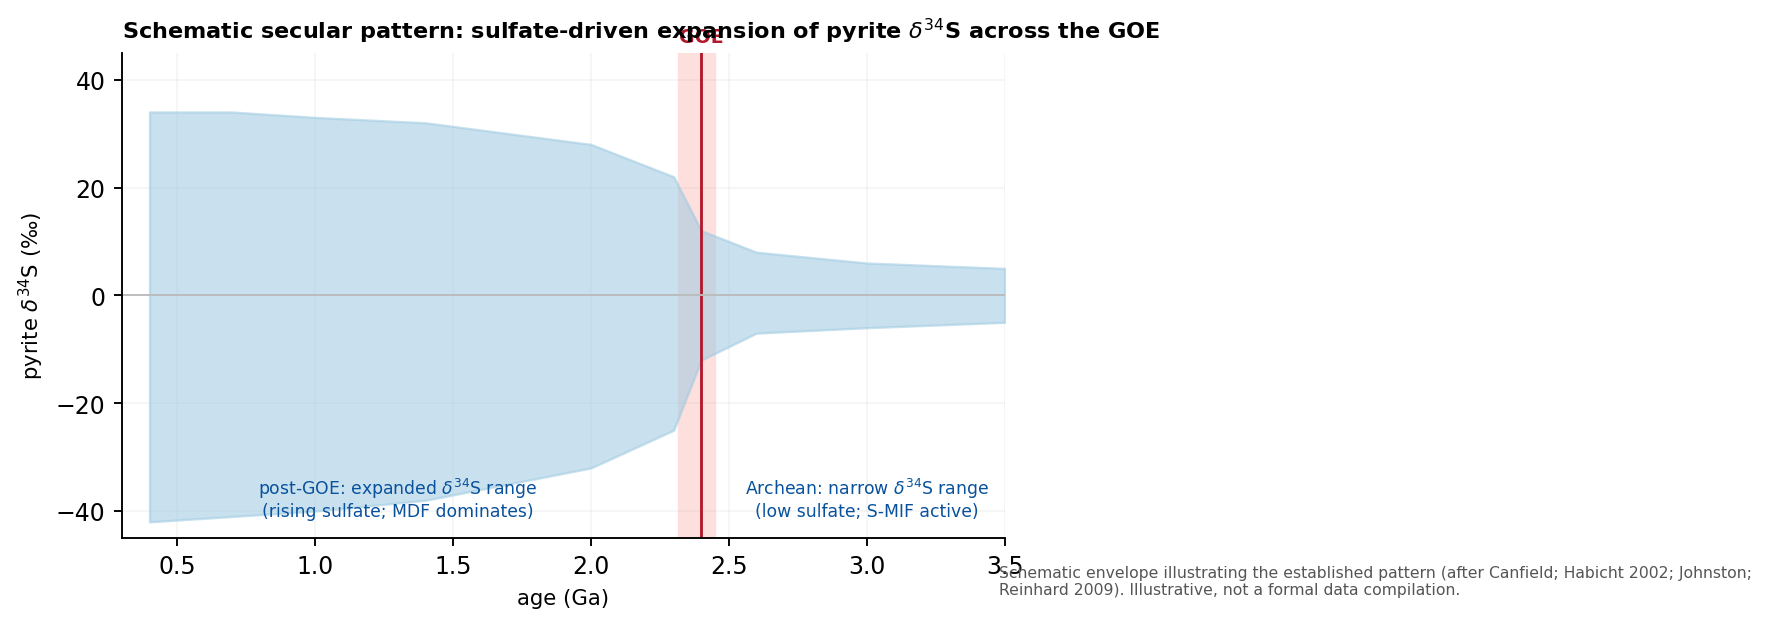
\includegraphics[width=\linewidth]{fig_v3_d34s.png}
\caption{Schematic secular pattern of pyrite $\delta^{34}$S (after \citealp{Canfield1998,Habicht2002,Reinhard2009,NeoarchS2017}). Illustrative envelope of the established pattern: a narrow Archean range expands
across the GOE as sulfate rises and mass-dependent fractionation dominates. Not a formal data
compilation.}
\label{fig:d34s}
\end{figure}

This confirms three things. (1) The GOE's sulfate rise is \emph{real} and recorded in
$\delta^{34}$S, so the second-order channel we invoked is not fictitious. (2) It began before the
GOE, so it is not cleanly GOE-gated. (3) It operates on the organic-matter decay/sulfurisation
balance---the S-rich versus S-poor kerogen pools documented in Tumbiana stromatolites
\citep{Lepot2009}---that is, on \emph{what} organic matter survives, not on the silicification-gated
\emph{morphological} fidelity that is this study's target. The channel is therefore real but
orthogonal to the morphological record. This refines the conclusion rather than rescuing a GOE
control on morphology: the GOE demonstrably reshaped sulfur cycling and organic-matter
sulfurisation, but that effect does not propagate into the morphological fossil pattern, which
remains silicification-controlled.

%==================================================================
\section{Formal within-formation test and power}

The within-formation Gunflint result motivates a direct per-sample test: regress MFI on SPI for
individual microfossil populations within single formations, controlling for thermal maturity (Raman
$R_2$), predicting a positive MFI$\sim$SPI slope significant within formations and sharing an
intercept across maturity-matched pre/post-GOE units. $\sim$30--50 populations per formation would
detect a moderate effect ($r\sim0.5$) at $\alpha=0.05$, power 0.8. This converts the contested
two-group pre/post-GOE contrast into a common-slope test that is both more powerful and more
mechanistically informative.

%==================================================================
\section{Revised interpretation (refined)}
The quantitative indices, the within-formation anchor, the unmasking analysis, and the
second-order-channel test jointly refine the conclusion. The GOE is not the primary control on
microfossil morphological preservation; silicification is, and silica capacity was high throughout
the Precambrian, so fidelity is gated by which facies received early silicification. The GOE
\emph{does} have a real taphonomic influence, but it is second-order, predates the GOE itself, and
confined to organic-matter sulfurisation and decay---which affects kerogen chemistry, not cellular
morphology. The post-GOE ``rise'' of microfossils is most parsimoniously a facies/sampling signal
amplified by well-exposed, well-sampled silica-encapsulating cherts, not an oxygenation signal; and
the unmasking--evolution question remains open precisely because the record is unreliable for that
biological inference.

%==================================================================
\section{Implications}
Treating microfossil abundance/diversity across the GOE as a direct biomass or biological-innovation
proxy is unreliable without facies/silicification correction; the molecular-clock-to-fossil gaps
warn against reading first appearances as origins. For biosignature search (early Earth, Mars), the
requisite variable for morphological preservation is a silica-encapsulating facies, not oxygen.

%==================================================================
\section{Conclusions}
Version~3 addresses the two outstanding objections. The unmasking--evolution ambiguity cannot be
resolved from biomarkers (contaminated pre-GOE, \citealp{French2015}) or first appearances
(facies-biased); molecular clocks are consistent with some pre-GOE lineages but not decisive. The
GOE's residual second-order channel is real---$\delta^{34}$S records the sulfate rise---but began in
the Neoarchean and acts on organic-matter sulfurisation, not on morphological fidelity. Both
results refine, rather than overturn, the central conclusion: morphological preservation is gated by
silicification (a facies variable, capacity high throughout the Precambrian), not by oxygenation;
the post-GOE ``rise'' of microfossils is best read as a facies/sampling signal; and the GOE's
taphonomic footprint is a second-order, OM-chemical one that does not map onto the morphological
record. A power-justified within-formation MFI$\sim$SPI test is the next empirical step.

%==================================================================
\bibliographystyle{plainnat}
\begin{thebibliography}{99}\footnotesize\linespread{0.92}\selectfont\setlength{\itemsep}{0pt}\setlength{\parskip}{0pt}
\bibitem[Alleon et al.(2016)]{Alleon2016silica} Alleon, J., et al. (2016). Early entombment within
silica minimizes the molecular degradation of microorganisms during advanced diagenesis.
\textit{Chemical Geology}.
\bibitem[Alleon et al.(2016a)]{Alleon2016} Alleon, J., et al. (2016). Molecular preservation of
1.88~Ga Gunflint organic microfossils as a function of temperature and mineralogy. \textit{Nature
Communications} 7, 11977.
\bibitem[Bekker et al.(2004)]{Bekker2004} Bekker, A., et al. (2004). Dating the rise of atmospheric
oxygen. \textit{Nature} 427, 117--120.
\bibitem[Betts et al.(2018)]{Betts2018} Betts, H.~C., et al. (2018). Integrated genomic and fossil
evidence illuminates life's early evolution and eukaryote origins. \textit{PNAS}.
\bibitem[Brocks et al.(1999)]{Brocks1999} Brocks, J.~J., et al. (1999). Archean molecular fossils
and the early rise of eukaryotes. \textit{Science} 285, 1033--1036.
\bibitem[Brocks et al.(2003)]{Brocks2003} Brocks, J.~J., et al. (2003). A hydrocarbon biomarker
perspective on the Archean atmosphere. \textit{Geochim. Cosmochim. Acta}.
\bibitem[Canfield(1998)]{Canfield1998} Canfield, D.~E. (1998). A new model for Proterozoic ocean
chemistry. \textit{Nature} 396, 450--453.
\bibitem[Crowe et al.(2014)]{Crowe2014} Crowe, S.~A., et al. (2014). Sulfate was a trace constituent
of the Archean ocean. \textit{Science} 346, 735--739.
\bibitem[Decreane et al.(2021)]{Decreane2021} Decreane, S., et al. (2021). Intense biogeochemical
iron cycling in Neoarchean Tumbiana Formation stromatolites. \textit{GCA}.
\bibitem[Delarue et al.(2020)]{Delarue2020} Delarue, F., et al. (2020). Out of rock: preservation of
microfossils from the 3.46~Gyr-old Strelley Pool Formation. \textit{Precambrian Research} 336, 105472.
\bibitem[Delarue et al.(2021)]{Delarue2021} Delarue, F., et al. (2021). Microfossils with tail-like
structures in the Strelley Pool Formation. \textit{Organic Geochemistry}.
\bibitem[Eme et al.(2014)]{Eme2014} Eme, L., et al. (2014). On the age of eukaryotes: evaluating
evidence from fossils and molecular clocks.
\bibitem[Farquhar et al.(2000)]{Farquhar2000} Farquhar, J., Bao, H., \& Thiemens, M. (2000).
Atmospheric influence of Earth's earliest sulfur cycle. \textit{Science} 289, 756--758.
\bibitem[French et al.(2015)]{French2015} French, K.~L., et al. (2015). Reappraisal of hydrocarbon
biomarkers in Archean rocks. \textit{PNAS} 112, 5915--5920.
\bibitem[Gardu\~{n}o Ruiz et al.(2024)]{Garduno2024} Gardu\~{n}o Ruiz, D., Goldblatt, C., \& Ahm,
A.-S.~C. (2024). Climate variability leads to multiple oxygenation episodes across the GOE.
\textit{Geophys. Res. Lett.} 51, e2023GL106694.
\bibitem[Habicht et al.(2002)]{Habicht2002} Habicht, K.~S., et al. (2002). Calibration of sulfate
levels in the Archean ocean. \textit{Science} 298, 2372--2374.
\bibitem[Hodgskiss \& Sperling(2020)]{Hodgskiss2020} Hodgskiss, M.~S.~W., \& Sperling, E.~A. (2020).
Stratigraphy and shale geochemistry of the Belcher Group.
\bibitem[Homann et al.(2015)]{Homann2015} Homann, M., et al. (2015). Morphological adaptations of
3.22~Ga-old tufted microbial mats, Moodies Group. \textit{Precambrian Research}.
\bibitem[Kah et al.(2004)]{Kah2004} Kah, L.~C., Lyons, T.~W., \& Frank, T.~D. (2004). Low marine
sulfate and protracted oxygenation of the Proterozoic biosphere. \textit{Nature} 431, 834--838.
\bibitem[Lepot et al.(2009)]{Lepot2009} Lepot, K., et al. (2009). Organic matter heterogeneities in
2.72~Ga stromatolites. \textit{Geochim. Cosmochim. Acta} 73, 6579--6599.
\bibitem[Lepot et al.(2017)]{Lepot2017} Lepot, K., et al. (2017). Iron minerals within specific
microfossil morphospecies of the 1.88~Ga Gunflint Formation. \textit{Nature Communications} 8, 14890.
\bibitem[Lyons et al.(2014)]{Lyons2014} Lyons, T.~W., Reinhard, C.~T., \& Planavsky, N.~J. (2014).
The rise of oxygen in Earth's early ocean and atmosphere. \textit{Nature} 506, 307--315.
\bibitem[Moore et al.(2025)]{Moore2025} Moore, K.~D., et al. (2025). Silicification of microfossils
as a taphonomic process (Cretaceous chert). \textit{Geobiology}.
\bibitem[Neoarchean S isotopes(2017)]{NeoarchS2017} Sedimentary sulfur isotopes and Neoarchean ocean
oxygenation (2017). \textit{Science Advances} 3, e1701835.
\bibitem[Pavlov \& Kasting(2002)]{Pavlov2002} Pavlov, A.~A., \& Kasting, J.~F. (2002).
Mass-independent fractionation of sulfur isotopes in Archean sediments. \textit{Astrobiology} 2, 27--41.
\bibitem[Perry \& Lefticariu(2003)]{Perry2003} Perry, E.~C., \& Lefticariu, P. (2003). Formation and
geochemistry of Precambrian cherts. \textit{Treatise on Geochemistry} 7, 99--113.
\bibitem[Philippot et al.(2018)]{Philippot2018} Philippot, P., et al. (2018). Globally asynchronous
sulphur isotope signals require re-definition of the Great Oxidation Event. \textit{Nature
Communications} 9, 2245.
\bibitem[Poulton \& Canfield(2005)]{Poulton2005} Poulton, S.~W., \& Canfield, D.~E. (2005).
Development of a sequential extraction procedure for iron. \textit{Chem. Geol.} 214, 209--221.
\bibitem[Poulton \& Canfield(2011)]{Poulton2011} Poulton, S.~W., \& Canfield, D.~E. (2011).
Ferruginous conditions: a dominant feature of the ocean through Earth's history. \textit{Elements}
7, 107--112.
\bibitem[Rasmussen et al.(2008)]{Rasmussen2008} Rasmussen, B., et al. (2008). Challenge to the
syngeneity of Archean hydrocarbon biomarkers (Pilbara craton). \textit{Nature}.
\bibitem[Reinhard et al.(2009)]{Reinhard2009} Reinhard, C.~T., et al. (2009). A late Archean sulfidic
sea stimulated by early oxidative weathering. \textit{Science}.
\bibitem[Sanchez-Baracaldo et al.(2021)]{Sanchez2021} Sanchez-Baracaldo, P., et al. (2021). The
Archean origin of oxygenic photosynthesis and extant cyanobacteria.
\bibitem[Shih et al.(2017)]{Shih2017} Shih, P.~M., et al. (2017). Crown group oxyphotobacteria
postdate the rise of oxygen. \textit{PNAS}.
\bibitem[Siever(1992)]{Siever1992} Siever, R. (1992). The silica cycle in the Precambrian.
\textit{Geochim. Cosmochim. Acta} 56, 3265--3272.
\bibitem[Sperling et al.(2014)]{Sperling2014} Sperling, E.~A., et al. (2014). Redox heterogeneity of
subsurface waters in the Mesoproterozoic ocean. \textit{Geobiology}.
\bibitem[Sugitani et al.(2010)]{Sugitani2010} Sugitani, K., et al. (2010). Biogenicity of
morphologically diverse carbonaceous microfossils from the $\sim$3.4~Ga Strelley Pool Formation.
\bibitem[v.1(2026)]{v1} [Author] (2026). Compiled-record test, Version 1. GEODISC study report.
\bibitem[v.2(2026)]{v2} [Author] (2026). Compiled-record test with operational indices, Version 2.
GEODISC study report.
\bibitem[Wacey et al.(2012)]{Wacey2012} Wacey, D., et al. (2012). Taphonomy of very ancient
microfossils, Strelley Pool and Gunflint formations. \textit{Precambrian Research}.
\bibitem[Wacey et al.(2013)]{Wacey2013} Wacey, D., et al. (2013). Nanoscale analysis of pyritized
microfossils in the $\sim$1.9~Ga Gunflint chert. \textit{PNAS} 110, 8020--8024.
\end{thebibliography}

\end{document}
